\documentclass[journal=jacsat,manuscript=article]{achemso}

\usepackage[version=3]{mhchem} % Formula subscripts using \ce{}
\usepackage[T1]{fontenc}       % Use modern font encodings
\usepackage{siunitx}
\DeclareSIUnit\Molar{\textsc{m}}
% !TeX root = ./azurin.tex
\usepackage{xr} 
\externaldocument{Sup_info}
\newcommand*\mycommand[1]{\texttt{\emph{#1}}}

\author{Authors}
\affiliation{Huygens-Kamerlingh Onnes Laboratory, Leiden University, RA, Leiden, The Netherlands}
\email{corresponding_author@physics.leidenuniv.nl}
\title[]
{A single azurin reveals intermolecular, intramolecular electron transfer and dynamic turnovers.}

\abbreviations{FCS}
\keywords{American Chemical Society, \LaTeX}

\begin{document}
%%%%%%%%%%%%%%%%%%%%%%%%%%%%%%%%%%%%%%%%%%%%%%%%%%%%%%%%%%%%%%%%%%
%%%%%%% Start the main part of the manuscript here.%%%%%%%%%%%%%%
%%%%%%%%%%%%%%%%%%%%%%%%%%%%%%%%%%%%%%%%%%%%%%%%%%%%%%%%%%%%%%%%%%
\section{Introduction}
Introduction here.
%%%%%%%%%%%%%%----------EXPERIMENTAL SECTION----------%%%%%%%%%%%%%%%%%%%%
\section{Experimental Section}
\subsection{Protein synthesis}
Azurin (wild type) from Pseudomonas aeruginosa was expressed in E. Coli and purified as described before \citep{kamp1990purification}. BL21 E.coli was transformed with PGK22 plasmid that has gene for azurin expression. The cells were cultured in luria broth (LB) medium. Then the cells were harvested and resuspended in 20 \% (w/v) sucrose solution in Tris pH 8 buffer containing 1 mM EDTA.Then the solution was centrifuged at 8000 rpm and the supernatant was collected. Copper sulfate was added to the solution for insertion into the active site of azurin. The unwanted proteins were precipitated by addition of acetic acid until pH 4. Again the turbid solution was centrifuged to separate azurin that remained in the supernatant. The azurin solution was loaded on a CM Sepharose fast flow column and elution was performed in an Akta purifier (GE Healthcare) with a pH gradient from 4 to 6.9 in 50 mM ammonium acetate. Fractions containing azurin collected and reduced with sodium dithionite. At this moment the solution both zinc and copper azurin. The azurins were purified in a DEAE sepharose column by a salt gradient of 0 to 50 mM NaCl in Tris pH8 buffer. Fractions containing copper azurin and zinc azurin collected and concentrated separately. The purity of the samples were checked by sodium dodecyl sulphate (SDS)-polyacrylamide gel electrophoresis (PAGE) and UV/Vis spectroscopy (Cary 50 spectrophotometer, Varian Inc., Agilent Technologies, USA). The azurins appeared on SDS gel page at \~14 kDa. Both zinc and copper azurin showed a characteristic peak at \~290 nm while Cu azurin showed an additional broad absorption peak at $620 nm$ as can be seen in figure S\ref{SIfig: switching} when oxidized. The ratio $O.D_{628 nm}/O.D_{280}$ for Cu azurin was 0.56 which indicated that all the azurin molecules had a Cu atom. The concentrated protein was stored at $-80^0 C$ until further use.
\subsection{Fluorescent labeling}
The labeling protocol was based on the previous work \cite{nicolardi2012topdown}. ATTO 655 NHS-ester was bought from ATTO-TEC GmbH. The buffer containing azurin was replaced with HEPES pH 8.3 and all the amine containing impurities were removed. A mixture of 200 $\mu$M azurin and ATTO 655 NHS-ester (ration 1:1) was incubated for 45 min. The NHS-ester group reacts to one of the amine group on the protein. The unreacted dyes were removed by a HiTrap desalting column. The labeled protein was concentrated in Tris pH 8.5 buffer by centrifuging in a 3 kDa Amicon ultra filter. The labeled protein further purified by an ion exchange chromatography in a 1 mL MonoQ column (GE Health). The different peaks obtained (see figure S\ref{SIfig: peak_sep}) corresponds to the different number and position of the dye on azurin. The peak-III corresponds to the protein labeled at Lysine122 position \cite{nicolardi2012topdown}. For this position of the dye, the protein construct shows high fluorescence switching (90 \%) ratio between oxidized and reduced condition as can be seen in Figure S\ref{SIfig: peak_sep}. This fraction was choosen for our single-molecule experiment as the two states can be observed easily. The same protocol was used for Zn azurin labeling and similar peak separation observed. The fluorescent labeled protein was then reacted with biotin-peg-NHS (MW 3400) in PBS pH 7.4 buffer with a ratio 1:5 to make sure each protein has at least one biotin. The free biotin was then remove centrifuging in a 3kDa Amicon ultra filter. The biotin on the protein will be used for immobilization on glass surface.
\subsection{Functionalization of cover slip}
Glass coverslips (Menzel-Glaser, 22mm × 40 mm, no. 1 thickness) were used for immobilization.The cover slips were sonicated in water (15 min) and acetone(15 min). Then they were rinsed in Milli-Q water several timesand incubated in a H2O/NH4OH/H2O2(5:1:1) bath at \SI{70}{\celsius}. The coverslips were rinsed several times with water and ethanol and finally stored in ethanol. Before functionalization, the slides were flamed. Then they were treated for 30 min with a 1\% solution of [3-(2-aminoethyl)aminopropyl]trimethoxysilane in methanol containing 5\% glacial acetic acid. This results in the binding of the active hydroxyl groups. The silane is not yet covalently bound. This is obtained by baking the cover slips in an oven at \SI{65}{\celsius} for 3 hours. After this treatment, the cover slips were sonicated for 10 minutes and washed with methanol. Dried with clean nitrogen, they were left in a desiccator overnight. The next day they were treated with a mixture of 5 mg/mL methoxy-peg-N-hydroxysuccinimide (MW 2000, Laysan Bio) and 0.05 mg/mL
biotin-peg-N-hydroxysuccinimide (MW 3400, Laysan Bio) in 50 mM phosphate buffered saline (PBS) with pH 7.4. This creates a surface containing biotin and methoxy end groups. The biotin then will bind to the NeutrAvidin with the CuAz attached to it (next section). The slides were dried with gentle flow of nitrogen and stored in a desiccator until further use.
\subsection{Protein immobilization}
The functionalized glass slide was incubated with 20 mM PBS pH 7.4 buffer for 5 min. 100 nM of Neutravidin (Thermo Scientific) was incubated for another 15 min and then washed to remove unbound Neutravidin. 100 pM of the labeled protein was then incubated for 1 min to get isolated proteins (20 per \SI{100}{\micro\meter} area) on the functionalized glass surface. The unbound proteins were then removed by replacing with a fresh PBS buffer.
\subsection{Electrochemical-potential control}
Once the unbound proteins are removed, a new mixture containing 0.1 mM sodium ascorbate ($[C_6H_7O_6]^-Na^+$) and 0.2 mM potassium ferricyanide ($[Fe(CN)_6]^{3-}$) in 4 mL PBS pH 7.4 was added at the sample holder which were our initial oxidant and reductant. Electrochemical potential of the solution is obtained from the ratio of oxidant and reductant. The ratio of of oxidant and reductant were further controlled by a potentiostat (Model 800B Series Electrochemical Detector, CH Instruments). A platinum rectangular grid (the total length/ width of the grid is around 2.5 cm) was used as working electrode and pressed onto the sample slide with the help of a small glass slide. Not only is the pressure evenly applied on the grid, but also small confined volumes are formed where the sample slide and glass slide form the `floor' and `roof' and the platinum grid forms the `walls'. A part of the platinum grid was exposed to the solution. These confined volumes are in the order of nanoliters, which makes switching of elctrochemical potential of solution possible in a matter of minutes.
\subsection{Confocal Microscope}
Single-molecule measurements were carried out in a home built confocal microscope. The setup was equipped with $635$ nm pulsed diode laser (Power Technology, Little Rock, AR, USA) controlled by PDL 828 "Sepia II" (PicoQuant) at $40$ MHz repetition rate. the laser beam was passed through a narrow-band cleanup filter (Semrock LD01-640/8-25) and coupled a single-mode optical fiber to obtain a Gaussian beam profile. The output beam was collimated and reflected by a polychroic mirror (z488/633rpc) onto the back aperture of an oil immersion objective (NA=1.4, Olympus UPLSApo 100x). The sample holder with the glass slide and electrodes were mounted on a scanning stage (Physik Instrumente P-517.3CD) controlled by nanopositioning system (Physik Instrumente E-710.3CD). The epifluorescence light was collected back through the same objective and focussed on a \SI{50}{\micro\metre} pinhole for spatial filtering, then passed through an emission filter (z488/635m "dual"-band emission filter, Chroma). The fluorescence beam was re-collimated and focussed on single-photon avalanche photo diodes (SPCM AQRH-15, Perkin Elmer Inc., USA). The signal from the photo diode was recorded by a PicoHarp 300 (PicoQuant GmBH, Berlin, Germany) in time-tagged-time-resolved mode.
\subsection{Data recording}
A $20$ by $20$ \SI{}{\micro\metre}$^2$ area of the sample surface functionalized with sparsely distributed ATTO655-labeled Azurin was scanned with $50$ nm per pixel and with a dwell time of $1$ ms per pixel. A typical fluorescence intensity image can be seen in Scheme-\ref{sch:setup}. A constant potential of $200$ mV (oxidizing) was applied by the electrochemical analyzer and an image of the same area taken after $2$ min. Typically within one minute, the solution potential of the mixture of $0.1$ mM ascorbate and $0.2$ mM ferricyanide reaches the applied potential. Another image of the same area recorded at $0$ mV (reducing). The two images were compared to identify the molecules that switch on-off at the two potentials Scheme-\ref{sch:setup} (9 \& 10). The coordinates of the switching molecules were registered and an automatic recording was started. For each molecule, time traces were recorded for $30$ s at different potentials between $-100$ mV and $100$ mV. For observing dynamic of a single-molecule over longer period, time traces were recorded until the dye on it bleached or became dead. The Zn-azurin-ATTO655 was used used as a control which doesn't show switching it's intensity at the above two potentials and time traces were recorded at the same potentials as Cu-azurin.
\subsection{Data analysis}
All the measurements resulted a huge amount data ($1000$ time traces). Each time trace contains absolute arrival times of photons as well as arrival time with respect to excitation laser pulse. This enabled us to extract maximum information from the traces. To minimize human error and attain efficiency, codes were written (in python, matlab) to analyze all the trace exactly the same way. The code and data ca be found in the given link (will be provided during submission). Mainly three analysis were made on each trace. (i) Change points in the time traces were obtained using the changepoint algorithm\cite{watkins2005detection} kindly provided by Prof. Haw Yang (Princeton University, USA). This method is binning free and doesn't require any prior knowledge of the underline kinetics. It determines the location of intensity changes based on the photon arrival times and The algorithm is recursively applied through the whole trace to find all the changes. Bayesian information criterion is used to find the number of states. Two states were predicted from long time traces and many molecules (2500 changepoints each) with more than 90\% accuracy which was expected from FRET quenching mechanism and total signal that we have. For the rest of the traces, we set the number of states to be two in order to minimize the computation time. An example of change points and it's overlap with the real time trace can be seen in Figure-\ref{fig:timetrace}. (ii) Autocorrelation of the time traces were performed by using SymPhoTime(PicoQuant) software. (iii) Further analysis of changepoint output and autocorrelations were performed in Python. The details of the code including all the fitting functions can be found in the online repositories (will be provided during submission).
%Scheme
\begin{scheme}
	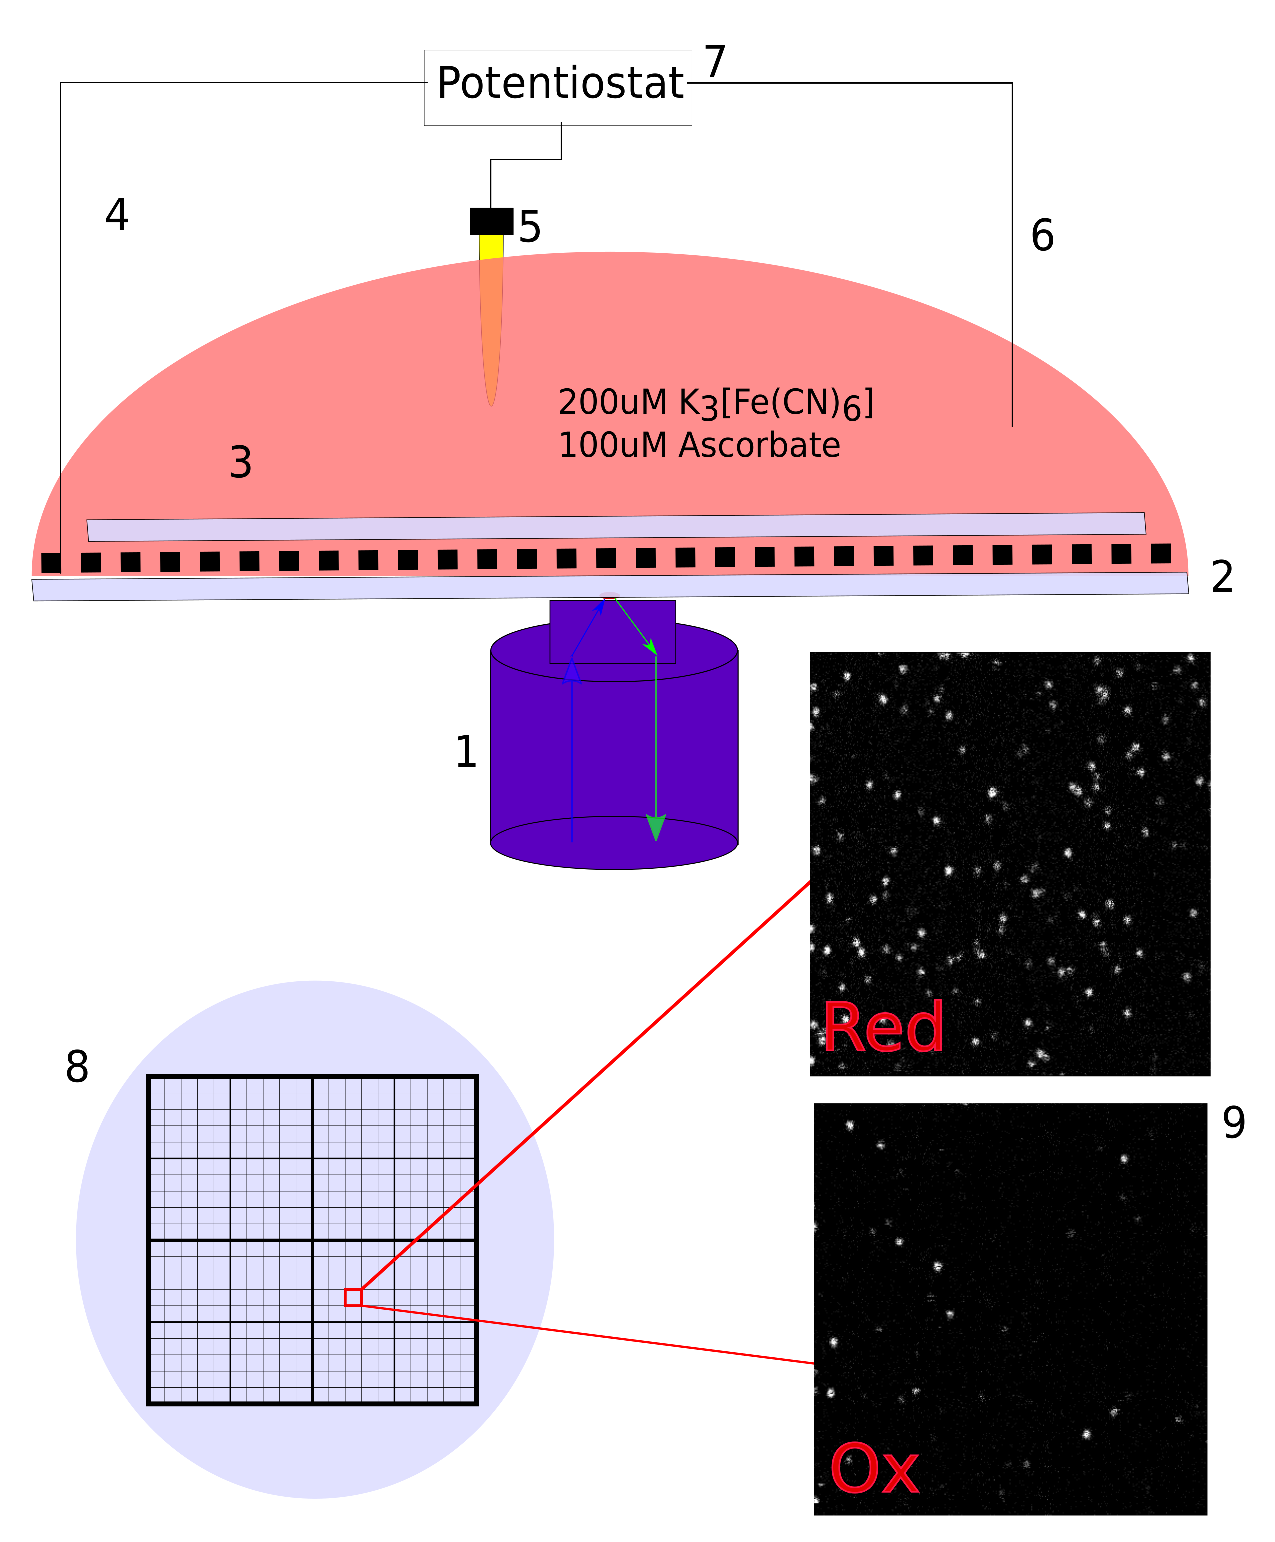
\includegraphics[scale=0.8]{Figure/Scheme_1_setup.eps}
	\caption{The scheme picture of the final setup. \textbf{(1)}  Objective through which light is irradiated on and collected from the sample. \textbf{(2)} The functionalized sample slide with on top the platinum grid
	and another small glass slide to press the grid on the sample slide, resulting in small confined volumes in the order of nanoliters. \textbf{(3)} The electron mediator solution consisting of \SI{200}{\micro\Molar} ferricyanide, \SI{100}{\micro\Molar} ascorbate in PBS (PH 7.4) buffer with a total volume of 4 mL. \textbf{(4)} The working electrode (Platinum wire) that is in contact with the platinum grid. \textbf{(5)} The saturated calomel reference electrode. \textbf{(6)} The Platinum wire (not touching the grid) as counter electrode. \textbf{(7)} The potentiostat (Model 800B Series Electrochemical Detector, CH Instruments) to which the electrodes are connected. \textbf{(8)}, \textbf{(9)} Top view of the sample slide and two images are showing the labeled Cu-Azurin reduced(brighter) and oxidized(dimmer).}
  	\label{sch:setup}
\end{scheme}
%%%%%%---------------------RESULTS and DISCUSSION-----------------------%%%%%%%%%
\section{Results and discussion\label{sec:results}}
\subsection{Time traces at different potentials}
Active Cu-azurin molecules were identified from their fluorescence intensity images at the oxidizing ($200~$mV) and reducing conditions($0~$mV). In reducing conditions, the image contains more brighter spots corresponding to Cu(I)-azurin-ATTO655 and more than $90~$\% of the molecules turned off in oxidizing conditions (Scheme-\ref{sch:setup}(9)). The azurins on each sample slide showed active switching during the course of our experiment (upto two days) without any noticeable degradation. A set of active azurins were marked for recording and time traces at different potentials (between 100 mV and -100 mV) were measured on the \texttt{same molecules} for $30~$s. Many of the labeled-protein bleached within recording at few potentials, but more than $50~$\% of the labeled-azurin survived atleast five measurements ($150~$s) at different potentials. Longer measurements were possible due to the scavenging of oxygen in the solution. Before the time trace recording, the solution was exposed to negative potential for at least $1~$hours. Ascorbate is known to  scavenge oxygen\cite{dave1997effectiveness} and get oxidized. The oxidized ascorbate is reduced by the electrode and was again available to scavenge other oxygen molecules. In addition to the absence of oxygen, the ROXS mechanism was also in play. The reduction and oxidation of Cu-azurin made the dye switch on and off, hence the fluorescent dye spent less time on the bright state where it is more prone to bleach. This made possible the measurement of some traces more than $1000~$s long.\\

Figure-\ref{fig:timetrace} shows time traces of a single Cu-azurin-ATTO655 at three different potentials. Clearly the intensity changes bright and dark over the time which is also schematically shown in the left of Figure-\ref{fig:timetrace} with the protein structure. The dark state is due to the FRET from the dye to the Cu(II) absorption center\cite{kuznetsova2006a}. Bulk measurements of the fluorescence intensity at completely oxidizing and completely reducing condition shows $90~$\% switching ratio (Figure-S\ref{SIfig: switching}) for the lysine-122\cite{nicolardi2012topdown} labeled Cu-azurin-ATTO655. Also single-molecule measurement (Figure-S\ref{SIfig: lifetime}) at a higher laser power (\SI{0.7}{\micro\watt}) shows more than $90~$\% switching which is consistent with the bulk measurements. The intensity of Cu(II)-state is lower than Cu(I)-stae, but higher than the background (bleached state). Also the Cu(II)-state has a shorter lifetime($0.3~ns$ than Cu(I)-state ($1.9~ns$), but longer than the instrument response function ($0.1~ns$). Both intensity and life time information reassure us that the dim-state we looking at is FRET quenched. Other blinking mechanism appears at lower potentials which will be discussed later. The high FRET efficiency is due to the small distance of the dye to the absorption center. This clear distinction between the on and off state was very important for our low laser power and lower signal measurement. At higher potential ($100~$mV), the protein spends most of the time in dark state and as the potential is lowered, the molecule spends more and more time on the bright state.
%time trace
\begin{figure}
	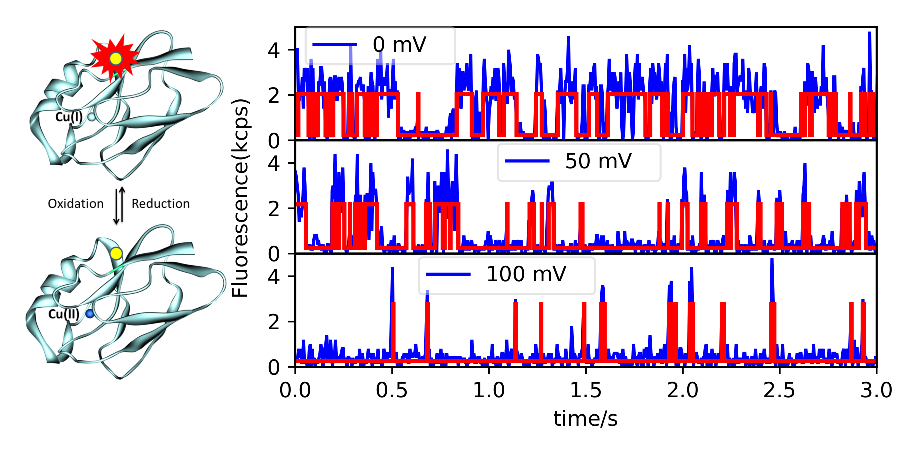
\includegraphics[width=\textwidth]{Figure/Figure_1_timetrace_CuAzu.eps}
	\caption{Time traces of Cu-Azurin labeled with ATTO655 at different potentials. The structure of the protein with properly positioned dye can be seen in the schematic picture in the left. In Cu(II) state (shown in bluish atom in the protein structure), the dye is non fluorescent because of FRET and in Cu(I) state (shown in gray atom), the dye is fluorescent. Notice the amount of time the protein spends on bright and dark state at different potentials. At lower potentials (e.g 0 mV) the protein is brighter most of the time because of the higher concentration of reductant.}
	\label{fig:timetrace}
\end{figure}
%Midpoint histogram
\subsection{Midpoint potential of single-azurins}
\begin{figure}
	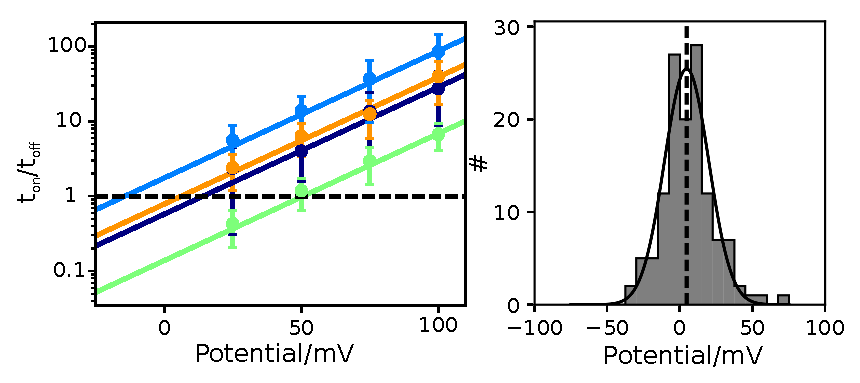
\includegraphics[width=\textwidth]{Figure/Figure_2_midpoint.eps}
	\caption{Ratio between on and off time as a function of applied potential for the same single-molecule. Different color represents different single-molecules. And the line connecting the data points is the Nernst fit for all the data points above 25 mV. The plot in the right is the histogram of midpoint potentials for $132$ molecules with a Gaussian fit with center 4.5 mV with respect to calomel electrode.}
	\label{fig:midpoint}
\end{figure}
%on-off 1D histogram
\subsection{Intermediate detection from on-off histogram}
\begin{figure}
	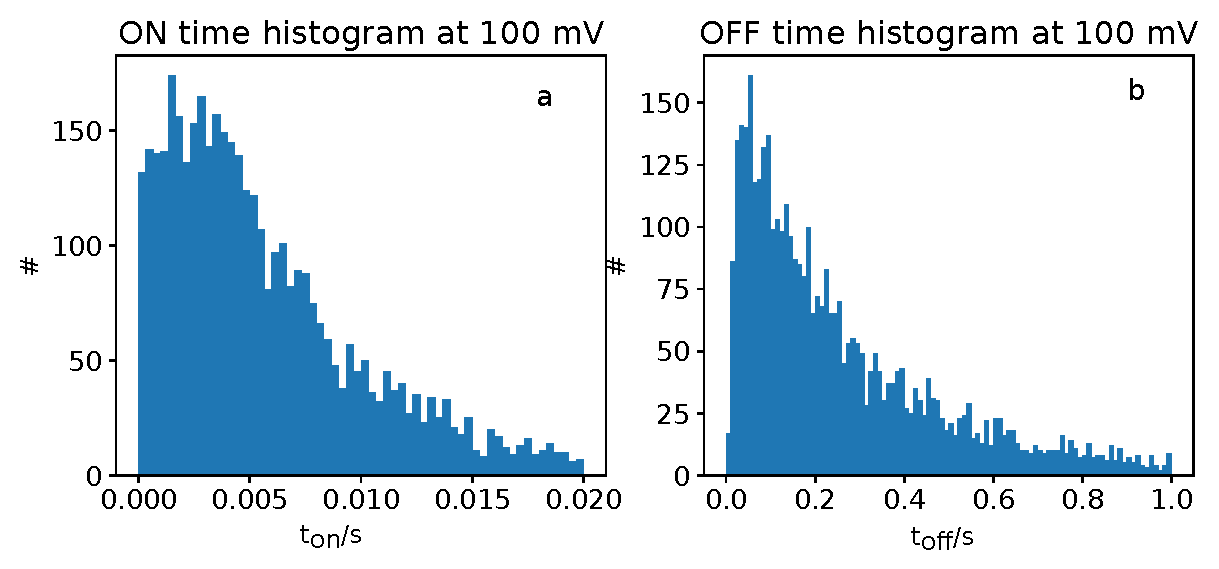
\includegraphics[width=\textwidth]{Figure/Figure_3_on_off_1D.eps}
	\caption{\textbf{On off histogram.} The histogram of on-times(a) and of off-times(b) of Cu-Azurin-ATTO655 showing rise time. This indicates that both oxidation and reduction of Cu-Azurin occurs through an intermediate step.}
	\label{fig:onoff1D}
\end{figure}
%Dynamic rates. protein showing diiferent rates with time
\subsection{Dynamics of ET rates}
\begin{figure}
	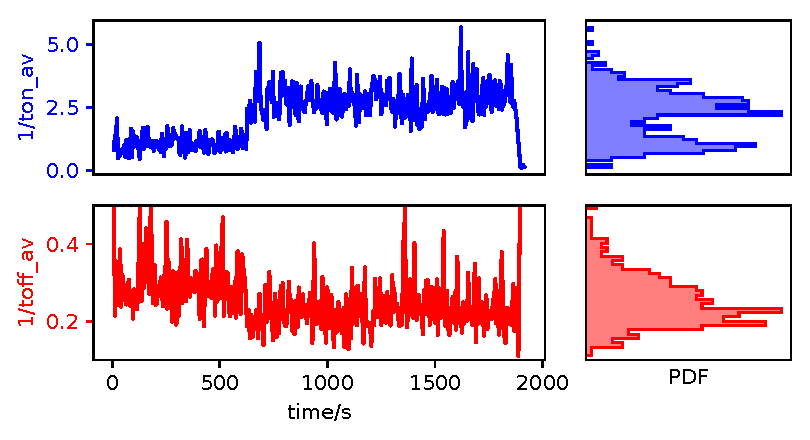
\includegraphics[width=\textwidth]{Figure/dynamic_rates.eps}
	\caption{\textbf{Dynamics in the turnovers of the protein.}}
	\label{fig:dynamic_rates}
\end{figure}
%Intramolecular electron transfer
\subsection{Intramolecular elctron transfer}
\begin{figure}
	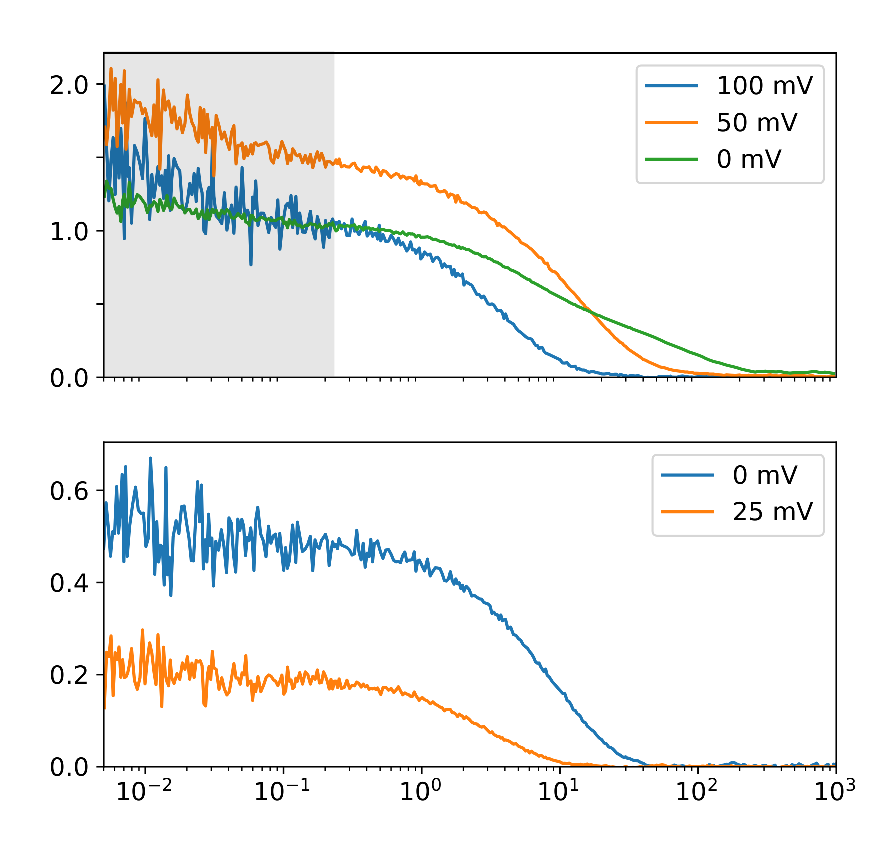
\includegraphics[width=\textwidth]{Figure/fcs_components.eps}
	\caption{\textbf{Intra molecular electron transfer.} Shorter decay with time constant of around 30 us}
	\label{fig:fcs_components}
\end{figure}
%on-off 2D histogram
\begin{figure}
	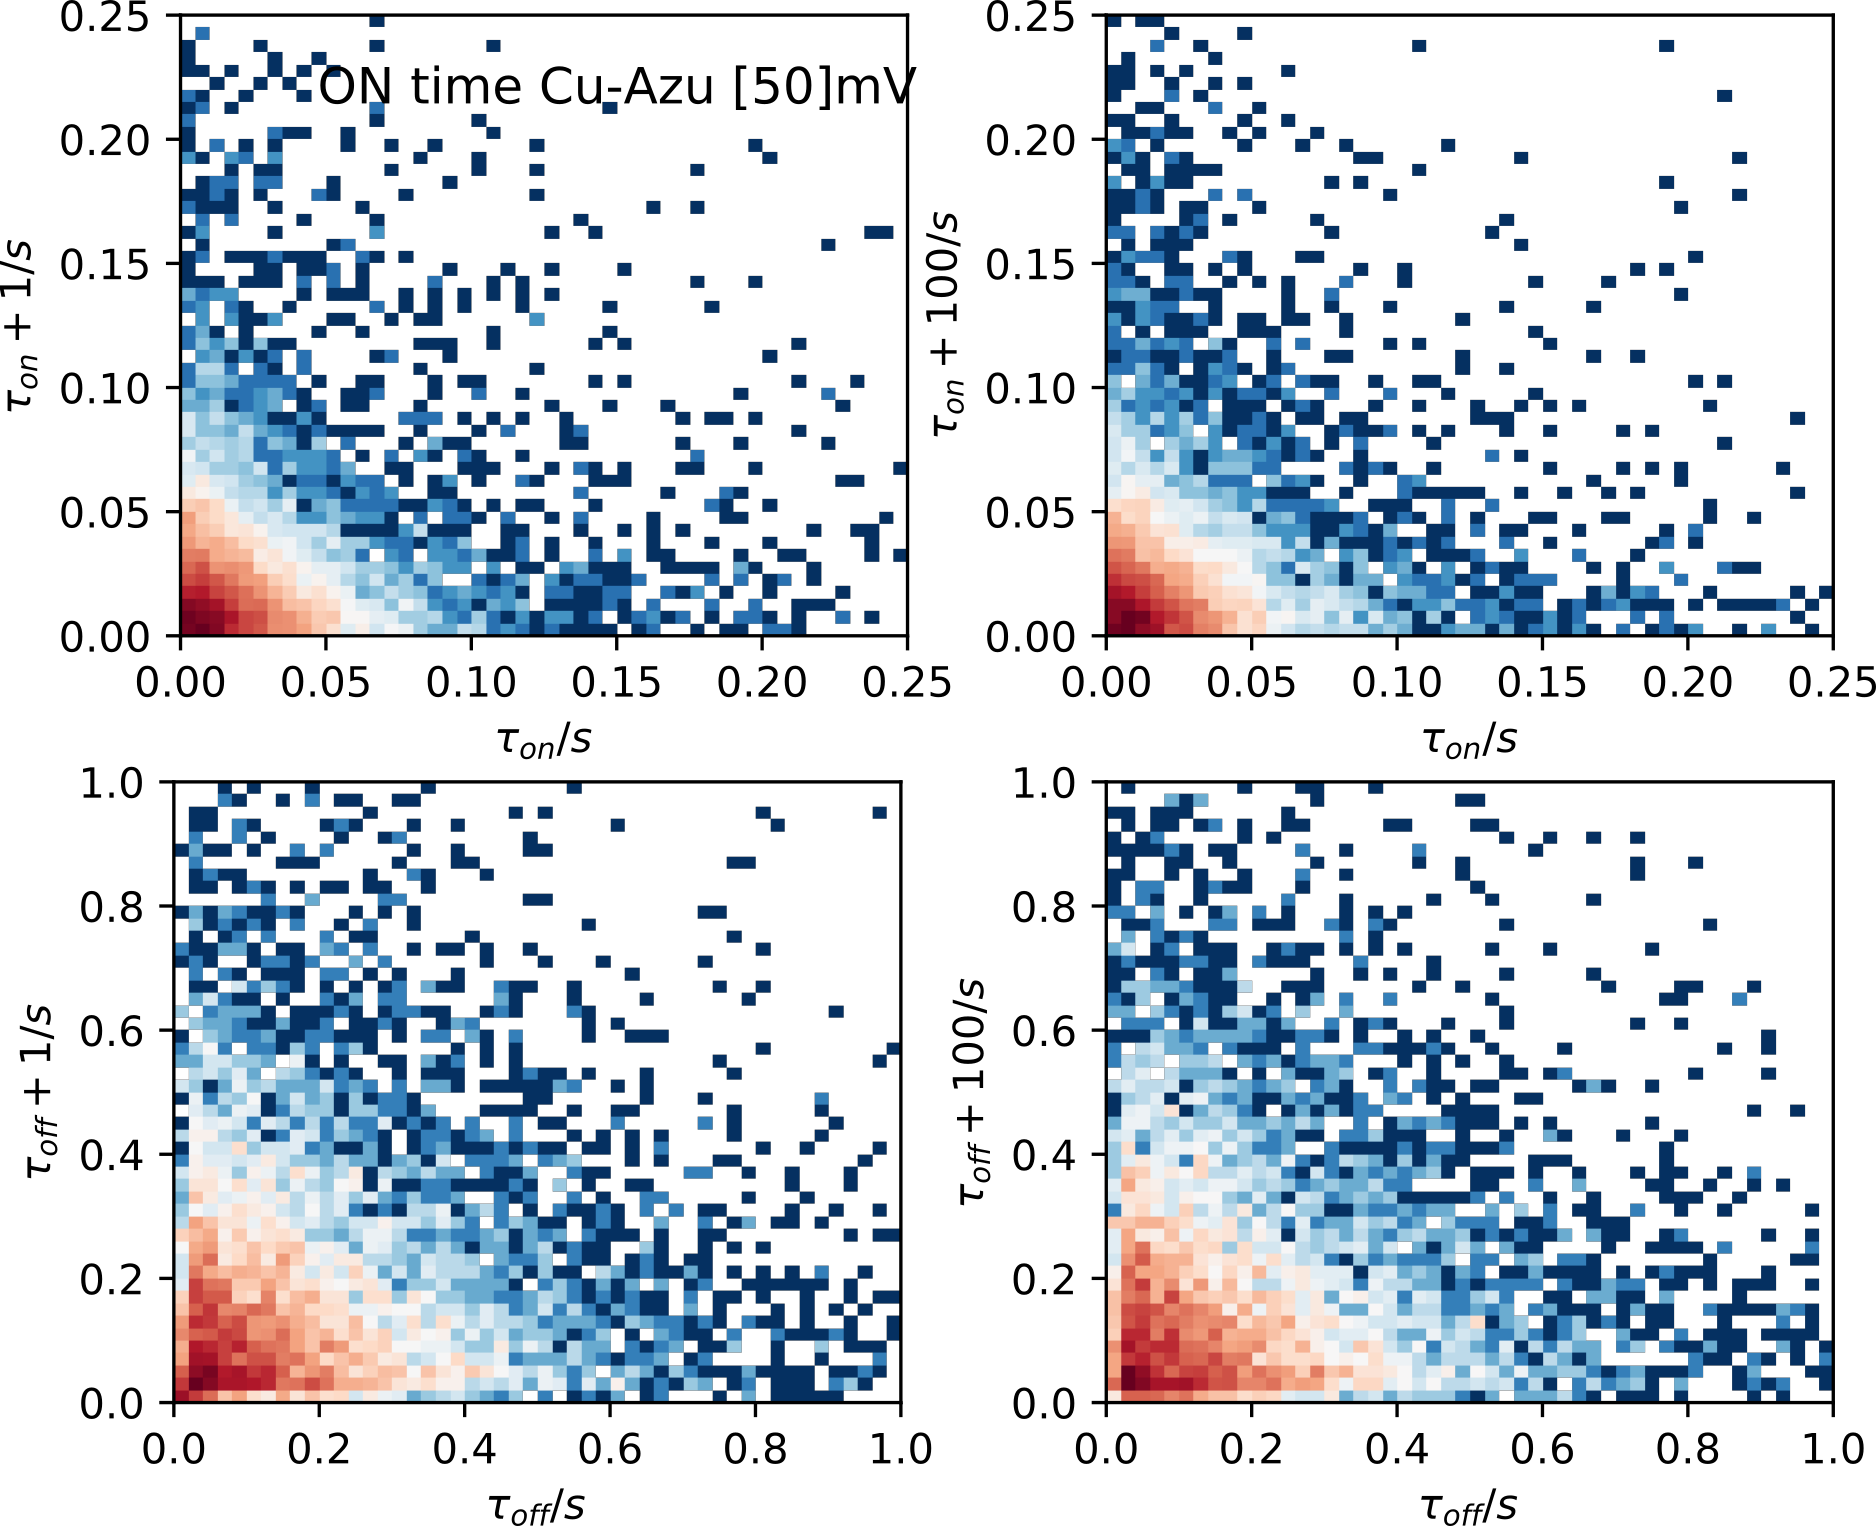
\includegraphics[width=\textwidth]{Figure/Figure_4_on_off_2D_100mV.png}
	\caption{\textbf{2D histogram: Cu-Azurin.} 2D correlation plot of (a) on-times vs the next on-times (b) on-times vs the on-time after 100 turnovers (c) off-times vs next off-times (d) off-times vs the off-time after 100 turnovers.}
	\label{fig:onoff2D}
\end{figure}
%%%%%Experimental Section%%%%%%%%%%
\section%{Experimental}
\bibliographystyle{achemso.bst}
\bibliography{azurin}
\end{document}